\documentclass[a4paper]{report}
\usepackage[utf8]{inputenc} 
\usepackage[romanian]{babel}
\usepackage{url}
\usepackage{a4wide}
\usepackage[bookmarks, bookmarksopen=true, bookmarksnumbered=true]{hyperref}
\usepackage{graphicx}
\linespread{1.5}
\addtolength{\parskip}{\baselineskip}

\renewcommand{\title}{OpenCad.org}
\newcommand{\subtitle}{Proiectarea unei aplicaţii CAD pentru arhitectură}
\renewcommand{\author}{Silviu-Georgian Aprozeanu}
\newcommand{\teacher}{prof. dr. ing. Florica Moldoveanu}

\newcommand{\col}[1]{@{\hspace{0.01\textwidth}}p{#1\textwidth}@{\hspace{0.01\textwidth}}}

\newtheorem{definition}{Definiţia}[chapter] 
\newtheorem{statement}{Propoziţia}[chapter]

\begin{document}
	\begin{titlepage}
\null \vfill
	\begin{center}
{\Huge \title{}}
	
{\Large \subtitle{}}
	\end{center}
\vfill
	\begin{flushright}
		\begin{tabular}{ll}
Absolvent & \author{} \\
Profesor îndrumător & \teacher{}
		\end{tabular}
	\end{flushright}
\vskip 2cm
	\begin{center}
\small Bucureşti, \today
	\end{center}
	\end{titlepage}
	\pagenumbering{roman}
\tableofcontents \listoftables \listoffigures \newpage
	\pagenumbering{arabic}
	\pagestyle{headings}
		�i-a�a-mi vine c�teodat�, doruleeee

�i-a�a-mi vine c�teodaaaat�, doruuuuule
S� dau cu cu�itu-n chiatr�,

S� dau cu cu�itu-n chiatr� doruuuule

		\chapter{Obiective}

Dintotdeauna am considerat că înainte de a iniţia orice activitate, fie că ea
este dezvoltarea unui produs software, fie că este orice altfel de sarcină de
amploare, autorul trebuie să-şi pună pe hîrtie o suită limitată de ţinte, nu
foarte uşor de realizat însă nu imposibile.

Pentru proiectul OpenCad.org, ele au fost alese prin perspectiva altor proiecte
similare dezvoltate în acest domeniu, şi am încercat să oferim ceva nou,
atractiv pentru eventualii utilizatori.

\section*{Uşurinţă în utilizare}

Dacă orice aplicaţie CAD tinde să ofere utilizatorilor ei unelte cît mai
puternice de dezvoltare, de multe ori se pierde din vedere ergonomia aplicaţiei.
Există un compromis ce trebuie făcut între capabilităţile aplicaţiei şi
ergonomie, însă nu credem că a cădea în oricare din tabere este benefic
rezultatului final al produsului.

De aceea, în realizarea acestui proiect am avut întotdeauna în vedere
interacţiunea cu utilizatorul şi interfaţa programului. Naturaleţea şi intuiţia
sunt cele mai bune metode de învăţare, şi nici o aplicaţie nu ar trebui să se
rezume la manualul sau documentaţia sa pentru a permite utilizatorilor să
înceapă să folosească această aplicaţie.

Noi ne-am dorit ca un utilizator să fie capabil să vadă rezultate efective
utilizînd aplicaţia noastră în cîteva minute după ce a deschis pentru prima dată
programul. Există multe aplicaţii CAD care necesită ore, dacă nu zile întregi de
acomodare cu setul de comenzi, setul de capabilităţi, de proprietăţi şi toate
celelalte componente ale unei aplicaţii de mare anvergură.

\section*{Puternică unealtă de dezvoltare}

Desigur, nu puteam ignora scopul final al activităţii de proiectare, şi anume
redarea cît mai fidelă a ideilor proiectantului. Dacă printr-o ergonomie
defectuasă acest deziderat poate fi împedicat prin încetinirea procesului, lipsa
totală a anumitor capacităţi de dezvoltare este cu atît mai dăunătoare
procesului de creaţie.

De aceea, în dezvoltarea acestui proiect am încercat în permanenţă să avem în
vedere toate facilităţile de care un proiectant ar avea nevoie pentru a-şi
realiza ideile sale, oferind funcţionalităţile necesare pentru a înlesni această
realizare.

\section*{Flexibilitate şi Extensibilitate}

Precum nu există o unealtă ce poate fi învăţată instantaneu, la fel nu există o
unealtă care să facă totul. Însă dorinţa noastră a fost a păstra aceste limite
superioare cît mai sus şi a oferi o gamă cît mai largă de servicii
utilizatorilor aplicaţiei de faţă.

În această privinţă, am încercat pe tot parcusul dezvoltării acestu produs ca un
viitor dezvoltator, fie el autorul sau o terţă parte, să poate porni de la o
bază solidă ce se constituie proiectul nostru şi să formeze mai departe o
unealtă mai puternică şi mai aproape de nevoile unor grupuri particulare de
utilizatori.

De departe, folosirea platformei Eclipse, despre care vom discuta în detaliu în 
cadrul Capitolului \ref{chapter:tech}, a facilitat într-o mare parte acest 
deziderat.
	\chapter{Tehnologii}
\label{chapter:tech}

\section{Eclipse Rich Client Platform}
\label{section:rcp}

Proiectul Eclipse îşi are începuturile alături de compania IBM de care s-a 
separat în 2003; astăzi este printre cele mai cunoscute proiecte opensource, 
fiind recunoscut ca un foarte popular mediu de dezvoltare de aplicaţii Java şi 
nu numai.

Binecunoscutul mediu de dezvoltare Eclipse este dezvoltat pe baza Eclipse Rich 
Client Platform. Aceasta reprezintă suita minimă de plugin-uri necesare pentru 
dezvoltarea unei aplicaţii "rich client" \footnote{eng. \textit{client bogat} 
-- O aplicaţie desktop care beneficiază de un set de elemente de interfaţă 
evoluate ("bogate"), care oferă o putere mare de abstractizare şi în acelaşi 
timp control al funcţionalităţii programatorului, păstrînd o experienţă de 
utilizare plăcută pentru utilizator. În general orice aplicaţie desktop care 
foloseşte elemente de interfaţă predefinite pînă la un anumit punct poate fi 
considerată ca un rich client.}. Deşi platforma este destinată dezvoltării de 
aplicaţii tip IDE, prin înlăturarea anumitor componente ale platformei se pot 
dezvolta orice tip de aplicaţii desktop.

Structura de bază a acestei platforme poate fi rezumată după cum am prezentat 
în Tabela \ref{table:rcpstruct}. \begin{table}[htp]
\caption{Structura Eclipse RCP \cite{rcpfaq} \label{table:rcpstruct}}
\begin{tabular}{|\col{0.23}|\col{0.73}|}
\hline Eclipse Runtime & Suport pentru plugin-uri, puncte de extensie şi 
extensii. Construită peste framework-ul OSGi\\
\hline SWT & Proiectat să ofere acces eficient şi portabil la facilităţile de 
interfaţă utilizator ale sistemului de operare pe care este implementat\\
\hline JFace & Un framework de interfaţă utilizator, construit pest SWT, pentru 
tratarea multor sarcini de programare de interfeţe\\
\hline Workbench & Construit peste toate componentele anterioare, aduce un 
mediu de lucru ultra scalabil, cu interfaţă publică ce suportă mai multe 
ferestre pentru administrarea vizualizărilor, editoarelor, perspectivelor, 
acţiunilor, preferinţelor şi multe altele. \\
\hline
\end{tabular}
\end{table}

\subsection{Eclipse Runtime. Equinox}
Această componentă a Eclipse RCP este cea mai abstractă şi în acelaşi timp cea 
mai puternică componentă a sa. Structura sa de bază este descrisă în Tabela 
\ref{table:runtimestruct}.

\begin{table}[htp]
\caption{Structura Eclipse Runtime \cite{eclipsehelp} \label{table:runtimestruct}}
\begin{tabular}{|\col{0.38}|\col{0.58}|}
\hline org.eclipse.core.contenttype & Suport pentru definirea şi administrarea 
tipurilor de fişiere \\
\hline org.eclipse.core.jobs & Infrastructură pentru programare paralelă în 
Eclipse \\
\hline org.eclipse.equinox.registry & Sistemul prin care un plugin publică alte 
plugin-uri de care depinde şi defineşte puncte de extensie pentru ca alte 
plugin-uri să-i îmbogăţească funcţionalitatea \\
\hline org.eclipse.equinox.preferences & O infrastructură prin care un plugin 
îşi păstrează preferinţele în seturi de perechi cheie/valoare modificabile de 
către utilizator \\
\hline org.eclipse.equinox.common & Administrarea proiectelor, resurselor şi 
fişierelor \\
\hline
\end{tabular}
\end{table}

\begin{quotation}
Equinox este o implementare a specificaţiilor OSGi R4
\footnote{\url{http://osgi.org/osgi_technology/download_specs.asp?section=2}}
o serie de plugin-uri care implementează diverse servicii opţionale OSGi şi 
alte infrastructuri pentru rularea sistemelor bazate pe OSGi. \cite{equinox}
\end{quotation}

\begin{quotation}
Equinox produce, printre alte lucruri, implementarea OSGi folosită de Eclipse 
RCP (şi celelalte proiecte bazate pe Eclipse) ca un model de componente.
\cite{equinoxfaq}
\end{quotation}

\begin{quotation}
OSGi este un framework care implementează un model de componente complet şi 
dinamic -- o componentă ce lipseşte din mediile Java. Aplicaţiile sau 
componentele (ce sunt sub formă de seturi de produse) pot fi instalate de la 
distanţă, oprite, pornite, aduse la zi şi dezininstalate fără a fi nevoie de 
repornirea aplicaţiei - administrarea claselor şi pachetelor Java este 
specificată în detaliu. Administrarea ciclului de viaţă este realizat prin 
interfeţe de aplicaţii care permit descărcarea la distanţă a politicilor de 
administrare. Registrul de servicii permite seturilor de aplicaţii să detecteze 
noi servicii, să detecteze dispariţia unor servicii şi adaptarea în consecinţă.

La început, proiectul s-a concentrat mai mult pe interfeţe de servicii dar s-a 
dovedit că aplicabilitatea este mult mai largă. Specificaţiile OSGi sunt 
folosite astăzi în aplicaţii pornind de la telefoane mobile pînă la Eclipse 
IDE. Alte aplicaţii includ automobile, automatizare industrială, automatizare 
în construcţii, PDA-uri, super-calculatoare, divertisment, administrarea 
flotelor şi servre de aplicaţii.

Specificaţia OSGi este creată de membri într-un proces deschis şi publicate 
fără taxe sub o licenţă specifică. Alianţa OSGi are un program de înscrieri 
care este deschis doar membrilor. Din ianuarie 2007, lista implementatorilor 
OSGi recunoscuţi conţinea 3 intrări.
\cite{osgiwiki}
\end{quotation}

Equinox este o implementare a specificaţiilor în versiunea 
R4, care conţine, printre altele\cite{osgiwiki}:

\begin{itemize}
  \item Noi capacităţi de modularizare puternince ce oferă încapsulare avansată 
  a serviciilor reţea care pot împărţi o singură maşină virtuală\footnote{O 
  maşină virtuală Java reprezintă o aplicaţie ce funcţionează ca un container 
  pentru toate aplicaţiile Java, oferind toate facilităţile unei maşini de 
  calcul ce ar putea executa nativ instrucţiuni Java.}.
  \item Partajarea claselor modularizată şi ascunderea detaliilor de 
  implementare.
  \item Tratarea avansată a diferitelor versiuni ale aceleaşi clase astfel 
  încît aplicaţiile noi pot fi executate în paralele cu cele noi în aceeaşi 
  maşină virtuală.
\end{itemize}

\subsection{SWT}
SWT\footnote{abrev. \textit{Standard Widget Toolkit}} este una din cele mai 
populare tehnologii dezvoltate de Fundaţia Eclipse. Această tehnologie 
foloseşte la crearea de interfeţe utilizator în mediul de dezvoltare Java, 
oferind programatorului capacitatea de a construi interfeţe utilizator 
portabile între diverse sisteme de operare. În prezent suportă toate sistemele 
de operare uzuale şi diverse arhitecturi maşină (e.g. x86, amd64).

Structura sa este similară cu cea a altor toolkit-uri similare, ca AWT 
\footnote{abrev. \textit{Abstract Window Toolkit} -- toolkit-ul IU standard 
Java \url{http://en.wikipedia.org/wiki/Abstract_Windowing_Toolkit}} şi 
SWING\footnote{Un toolkit IU independent de platformă 
\url{http://en.wikipedia.org/wiki/Swing_(Java)}}. Elementele fundamentale sunt 
Shell-ul şi Controlul. Un shell este abstracţia conceptului de fereastră şi 
reprezintă în general un container pentru controale. Controalele sunt 
elementele interfeţei utilizator. Butoanele, etichetele, arborii şi tabelele 
sunt toate controale şi utilizatorii sunt obişnuite cu ele din alte programe 
ale desktopului. \cite{swt} În principiu orice widget poate fi simplu sau 
compus (i.e. descendent al clasei Composite) şi întreaga lor ierharhie este 
controlată de relaţiile dintre clasele SWT.

Interacţiunile dintre controale şi utilizator cît şi controlul tranziţiei 
stărilor controalelor se face cu ajutorul Evenimentelor. Fiecare modificare de 
stare a unui control (cum ar fi apăsarea pe un buton) este semnalată de SWT 
către aplicaţie prin declanşarea unui eveniment. Orice Listener (ascultător 
înregistrat pentru un anumit eveniment) va primi o notificare (i.e. o metodă 
declarată în interfaţa de Listener va fi apelată) ce va conţine evenimentul ce 
a avut loc. Orice clasă poate deveni listener prin implementarea unor interfeţe 
specifice, SWT oferind astfel o mare flexibilitate în cadrul aplicaţiilor care 
îl folosesc.

Ca şi în AWT sau SWING, poziţia controalelor este stabilită cu ajutorul 
Layout-urilor. Un layout reprezintă un set de reguli de poziţionare pentru un 
control compus ce va decide pentru toate controalele incluse cum vor fi ele 
poziţionate pe ecran. Unele layout-uri asociază anumite date fiecărui control 
pentru a reţine poziţia în care va fi desenat. Poziţionarea manuală a tuturor 
controalelor este o problemă complexă şi dacă acel algoritm nu este scris 
eficient, el poate afecta performaneţele întregii aplicaţii. De aceea, SWT 
oferă nişte seturi predefinite de layout-uri ce serversc cele mai comune cazuri 
întîlnite de programatori.

\subsection{JFace}
JFace este un toolkit pentru interfeţe utilizator ce conţine clase pentru 
tratarea multora din sarcinile uzuale de programarea interfeţelor utilizator. 
JFace este independent de sistemul de ferestre atît in interfaţa sa pentru 
programatori cît şi în implementare, şi este proiectat să funcţioneze cu SWT 
fără a-i ascunde funcţionalitatea.

JFace include componentele uzuale de toolkit IU, regiştri de imagine şi seturi 
de caractere, text, dialog-uri, framework-uri pentru preferinţe şi wizard-uri
\footnote{Dialogurile des întîlnite ce automatizează diverse sarcini repetitive}
şi raportarea progresului pentru sarcini cu durată mare de execuţie.
\cite{jface}

Pachete principale din JFace, care oferă funcţionalitatea de bază a tehnologiei 
sunt prezentate în Tabela \ref{table:jfacestruct}.

JFace reprezintă un strat de abstractizare suplimentară faţă de SWT, ce
îmbunătăţeşte performanţa şi timpul de dezvoltare a interfeţelor vizuale
dezvoltate cu aceste tehnologii. JFace reprezintă o completare importantă a
setului SWT, ce aduce tehnologia dezvoltată de Eclipse la acelaşi nivel cu alte
framework-uri similare, cum ar fi .net Framework. Importanţa deosebită a acestei
extensii o reprezintă separarea totală de librăriile AWT şi SWING, care nu mai
sunt necesare nici măcar pentru administrarea imaginilor sau a fonturilor din
sistem.

\begin{table}[htp]
\caption{Structura JFace \cite{jface-art} \label{table:jfacestruct}}
\begin{tabular}{|\col{0.13}|\col{0.28}|\col{0.53}|}
\hline Ferestre & org.eclipse.jface.window & Facilităţi de creerea şi 
administrarea ferestrelor. Interesantă este clasa ApplicationWindow, care aduce 
un nou nivel de abstracţie peste conceptul de fereastră şi înglobează o buclă 
program SWT.\\
\hline Vizualizări & org.eclipse.jface.viewers & Vizualizări ca şi TreeViewer 
sau TableViewer, care sunt componente ghidate de model ce folosesc widgeturi 
SWT şi adaptează conţinutul modelului la conţinutul widgetului.\\
\hline Dialog-uri & org.eclipse.jface.dialogs & Diverse dialog-uri des 
folosite.\\
\hline Acţiuni & org.eclipse.jface.actions & Un framework de acţiuni IU similar 
cu cel găsit în SWING pentru a implementa comportament partajat între două sau 
mai multe componente, cum ar fi o intrare în meniu şi un buton de pe bara de 
instrumente.\\
\hline Wizard-uri & org.eclipse.jface.wizard & Un framework avansat de 
construcţie a wizard-urilor.\\
\hline Resurse & org.eclipse.jface.resource & Suport pentru administrarea 
resurselor, cum ar fi imaginile şi fonturile SWT.\\
\hline Text & org.eclipse.jface.text & Un framework de crearea, manipularea, 
afişarea şi editarea documentelor text.\\
\hline
\end{tabular}
\end{table}

\subsection{Workbench}
\label{section:workbench}
Această parte a Eclipse RCP reprezintă o colecţie largă de clase şi interfeţe 
pentru construirea de interfeţe utilizator complexe.

Iată principalele elemente ce constituie un Workbench.

\subsubsection{Workbench}
Ca termen strict, se referă la fereastra care conţine întreaga aplicaţie. 
Defineşte un container abstract pentru toate elementele de interfaţă din 
aplicaţia dezvoltată cu Eclipse RCP.

Funcţionalitatea sa programatică este să răspundă nevoilor abstrace, care nu
sunt legate în mod specific de interfaţa vizuală, deservind însă desigur şi
scopurilor ferestrei pe care o conţine.

\subsubsection{Pagina}
Reprezintă, în mod intuitiv,  toată partea ferestrei care nu conţine barele de 
unelte şi meniul.

Pagina reprezintă o colecţie de Părţi şi conţine în funcţionalitatea sa un
algoritm de gruparea a părţilor. O pagină reprezintă containerul atît fizic cît
şi la nivel al logicii aplicaţiei a tuturor părţilor. Ea comunică diverse
informaţii între aceste părţi pentru a le ajuta să-şi sincronizeze conţinutul.

\subsubsection{Perspective}
Folosesc pentru organizarea conţinutului într-o Pagină. O perspectivă defineşte 
o colecţie de Vizualizări, aşezarea lor şi acţiunile ce pot fi efectuate pentru 
o sarcină a utilizatorului. Perspectivele pot fi schimbate de către 
utilizatorul. Modificarea Perspectivei afectează doar Vizualizările nu şi 
Editoarele. \cite{eclipsehelp}

\subsubsection{Părţi. Vizualizările şi Editoarele}
Părţile sunt o abstracţie a editoarelor şi vizualizărilor, privite prin
perspectiva lor comună de componente ale unei pagini. Părţile au în comun o
serie largă de proprietăţi ce le ajută să comunice între ele la acest nivel
abstract la care există nevoia de sincronizare, de informare asupra stării
diverselor componente, etc.

Reprezintă extensiile aduse de programator într-o aplicaţie Eclipse RCP. Un 
editor urmăreşte modelul unei maşini de stări în sensul că el are o etapă de 
deschidere, editare şi o etapă de salvare.

În schimb orice modificare a stării unei Vizualizări este salvată imediat. 
Vizualizările sunt folosite la a arăta structura modelului deschis într-un 
Editor, la a facilita accesul la fişiere şi la alte resurse ale unui proiect.

Editoarele urmăresc în general modelul unui editor de text clasic şi oferă 
aceeaşi funcţionalitate însă la un nivel mai abstract, nefiind dependent de o 
intrare ca fişier text, nici măcar ca intrarea să fie orice fel de fişier.

\section{OpenGL şi extensia OpenGL pentru SWT}

OpenGL\footnote{abrev. \textit{Open Graphics Library}} este o specificaţie de 
standard independent de limbaj ce definieşte un API pentru scrierea de 
aplicaţii ce produc grafice tridimensionale sau bidimensionale pe calculator. 
Interfaţa este compusă din peste 250 de apeluri de funcţii ce pot fi folosite 
pentru a desena scene tridimensionale complexe din primitive simple. OpenGL a 
fost dezvoltat de SGI\footnote{abrev. \textit{Silicon Graphics Inc.}} în 1992. 
Este folosit pe scară largă în aplicaţii CAD, realitate virtuală, vizualizare 
ştiinţifică, vizualizarea informaţiei, simularea zborului, dezvoltare de jocuri 
pe calculator, ş.a. \cite{oglwiki}

\subsection{OpenGL în Java}
Java reprezintă una dintre cele mai puternice platforme de dezvoltare de 
aplicaţii cunoscute în ziua de azi. Dezvoltată iniţial pentru a separa sarcina 
de dezvoltare de aplicaţii de platforma pe care va rula, astăzi limbajul Java 
este folosit în numeroase aplicaţii software, începînd de la clienţi destop 
pînă la jocuri pentru telefoane mobile şi aplicaţii web. Un astfel de sistem nu 
putea să rămînă fără o implementare a OpenGL. În prezent, există două extensii 
OpenGL pentru Java, JOGL şi LWJGL.

JOGL\footnote{Java OpenGL Library \url{http://jogl.dev.java.net}} este varianta 
agreată de Sun şi urmează să facă parte din distribuţia oficială a 
JDK\footnote{După cum precizează JSR231 
\url{http://jcp.org/en/jsr/detail?id=231}}. Principala sa caracteristică este 
că foloseşte AWT ca şi suport de interfaţă grafică.

LWJGL\footnote{Lightweight Java Game Library \url{http://lwjgl.org/}} este o 
soluţie mai amplă dedicată dezvoltării de jocuri în OpenGL. Librăria oferă şi 
suport pentru tratarea sunetului şi a evenimentelor de interacţiune cu 
utilizatorul, specializate cum am spus după nevoile programării jocurilor pe 
calculator.

\subsection{OpenGL pentru SWT}

Din păcate, nici una din aceste tehnologii nu se împacă foarte bine cu SWT. 
Pentru că atît OpenGL cît şi SWT şi AWT implică apeluri native către sistemul 
de operare, de multe ori aceste apeluri sunt ignorante unele de celelalte şi 
multe interferenţe apar între interfaţa grafică desenată cu SWT şi fereastra de 
desenare OpenGL.

Din aceste raţiuni, o a treia variantă a fost aleasă de noi, anume extensia 
OpenGL pentru Java făcută de Eclipse pentru SWT. Este de menţionat că rezultate 
similare s-au obţinut şi LWJGL, care la rîndul său poate fi integrat cu puţin 
efort cu SWT. JOGL din păcate, datorită legăturii sale puternice cu AWT, nu 
poate fi adus în scopul aplicaţiei noastre într-un mod care să poate fi uşor 
reproductibil de autor.

Limitările bibliotecii OpenGL pentru SWT făcute de Eclipse se referă la 
versiunea de OpenGL suportată (i.e. OpenGL 1.1) şi la faptul că interesul 
pentru această tehnologie este oarecum scăzut, ultima versiune existentă 
datează din septembrie 2005\footnote{\url{http://www.eclipse.org/swt/opengl/}} 
şi sunt şanse ca versiuni ulterioare să nu mai existe, pe cînd celelalte două 
librării sunt în continuă dezvoltare.

La momentul determinării acestei alegeri, după o testare a tuturor 
tehnologiilor disponibile, am ajuns la concluzia că funcţionalitatea oferită de 
varianta Eclipse a legăturii cu OpenGL este atît suficientă ca şi capaciţăţi 
necesitate de acest proiect cît şi destul de stabilă pentru a oferi o calitate 
înaltă de producţie.

\section{Raţiunea alegerii tehnologiilor}

Încă de la începutul dezvoltării acestui proiect, s-a pus problema tehnologiei 
care să fie folosită pentru îndeplinirea cît mai facilă a obiectivelor 
proiectului. Munca de cercetare în privinţa alegerii tehnologiei potrivite a 
implicat o documentare amplă asupra tehnologiilor luate în considerarea cît şi 
testarea practică a multora dintre ele.

Vom încerca mai jos să trecem în revistă o serie de alegeri care le-am făcut şi 
raţiunea ce stă în spatele lor, prin prisma avantajelor şi dezavantajelor aduse 
de alegerile făcute.

\subsection{PHP şi Python}

Consideraţia asupra alegerii limbajului de programare în care urma să fie 
dezvoltat acest proiect a început desigur de la aria cunoştinţelor autorului. 
Alegerea s-a făcut astfel între C, C++ şi Java. Alte alternative mai 
``exotice'' au fost luate în considerare marginal, cum ar fi 
Python\footnote{\url{http://www.python.org/}} sau 
PHP\footnote{\url{http://www.php.net/}}.

Capacităţile limbajelor scripturale de a intercaţiona cu libării native şi de a 
crea interfeţe grafice a cunoscut o dezvoltare masivă în ultima perioadă. 
Există pentru Python PyGTK\footnote{\url{http://www.pygtk.org/}}, o librărie ce 
permite programarea facilă a intefeţelor grafice cu GTK\footnote{abrev. 
\textit{The GIMP Toolkit} \url{http://www.gtk.org/}} sub Python. O extensie 
similară există pentru PHP, numită PHP-GTK\footnote{\url{http://gtk.php.net/}}.

Din punctul de vedere al graficii tridimensionale, extensii similare există 
pentru ambele limbaje, oferind funcţionalitate similară cu extensia prezenză în 
limbajul Java.

La nivel de dezvoltarea de aplicaţii desktop complexe, pentru Python există 
framework-ul DABO\footnote{\url{http://dabodev.com/} Un framework orientat pe o 
funcţionalitate client similară aplicaţiei Visual FoxPro} bazat pe 
wxPython\footnote{\url{http://www.wxpython.org/} un framework similar cu 
wxWidgets (despre care vom discuta ulterior), ce oferă portabilitate pentru 
codul intefeţei grafice între diverse sisteme de operare}. Apropierea acestor 
sisteme de cerinţele noastre nu a fost evidentă, cît şi popularitatea relativă 
a acestor proiecte a făcut considerarea lor doar trecătoare.

\subsection{C şi C++}

Revenind la principalii candidaţi, limbajele tradiţionale pentru dezvoltarea de 
aplicaţii software nu puteau să treacă neobservate autorului. Există o suită 
impresionantă de aplicaţii desktop dezvoltate exclusiv doar pe baza acestor 
două limbaje de operare.

Ca şi set de widgeturi interesante pentru noi, menţionăm librăriile GTK, 
QT\footnote{\url{http://en.wikipedia.org/wiki/Qt_(toolkit)}} şi bineînţeles 
.NET Framework\footnote{\url{http://msdn.microsoft.com/netframework/}}.

Programarea la nivel de bază, cum este cea în limbajul C nu a fost niciodată 
agreată de autor pentru capacităţile limitate de scalare (sau viteza redusă de 
scalare şi efortul depus pentru scalare), lipsa unei integrări independente de 
platformă la un nivel superior şi cu o structură coerentă, orientată obiect.

Aceste considerente au cîntărit greu împotriva bibiliotecii GTK, cea mai 
populară arhitectură open-source de dezvoltare de aplicaţii grafice în C, ce 
stă la baza sistemului desktop GNOME\footnote{\url{http://www.gnome.org/}, un 
sistem destkop complet, întîlnit în majoritatea distribuţiilor Linux cît şi a 
majorităţii altor platforme UNIX}.

În contrabalans a stat librăria gtkmm\footnote{\url{http://www.gtkmm.org/}}, o 
extensie a lui gtk pentru C++. Pînă în ziua de astăzi, o despărţire clară de 
această tehnologie din partea autorului nu există. Unicele considerente 
împotriva acestei alegeri rămîn dependinţa de limbajul C++ şi lipsa unei 
portabilităţi între sisteme de operare de o stabilitate apreciabilă.

Răspunsul acestor lipsuri a părut să îl aibă 
wxWidgets\footnote{\url{http://www.wxwidgets.org/}}. O platformă cu o tradiţie 
considerabilă în dezvoltarea de aplicaţii client, wxWidgets reprezintă poate 
cea mai bună alegere pentru un dezvoltator de aplicaţii client portabile sub 
C++, în opinia noastră.

Însă o analiză mai profundă a acestei platforme a scos la iveală faptul că 
wxWidgets există ca şi sistem de dezvoltare de aplicaţii client dinaintea 
extensiei STL\footnote{abrev. \textit{Standard Template Library} 
\url{http://en.wikipedia.org/wiki/Standard_Template_Library}} pentru C++. De 
departe -- în opinia autorului -- cea mai atractivă componentă a limbajului C++ 
suferă de un suport consistent pentru wxWidgets.\cite{wxfaq} Această 
caracteristică a bibliotecii a reprezentat un criteriu de nedepăşit în alegerea 
noastră.

Biblioteca QT a trebuit să fie dată la o parte pe baza principiului 
portabilităţii. Din păcate, există puţine implementări de succes de software 
implementat cu QT pentru platforma Windows. De asemenea, QT nu este distribuit 
sub o licenţă compatibilă cu intenţiile de distribuţie ale autorului.

\subsection{.net Framework}

Dacă pînă acum ne-am uitat la tehnologii care pornesc dinspre domeniul 
open-source şi Linux, .net Framework reprezintă răspunsul gigantului Microsoft 
la evoluţia sistemelor software moderne.

Cu o structură de clase avansată, .net Framework este printre puţinele soluţii 
software atît de impresionante care nu au reuşit să-şi găsească un răspuns 
rezonabil în lumea opensource.

Deşi reprezintă ţelul unui întreg proiect, 
mono\footnote{\url{http://www.mono-project.com}}, la data la care am făcut 
cercetările noastre, portabilitatea sistemului .net pentru platforme UNIX nu a 
ajunsese încă, în opinia autorului, la o maturitate demnă de luat în seamă. 
Aflat într-o continuă dezvoltare, proiectul mono promite să realizeze o 
revoluţie în ceea ce priveşte portabilitatea programelor software pe diverse 
sisteme de operare.

\subsection{Java}

Dintre toate sistemele de dezvoltare software existente astăzi în lumea 
dezvoltatorilor de aplicaţii desktop, noi am decis că Java reprezintă cel mai 
convenabil, uşor de dezvoltat, uşor de menţinut şi uşor de distribuit mod de a 
dezvolta proiectul de faţă.

Cu o istorie legendară de realizări, Java reprezintă poate cel mai dezvoltat 
sistem software existent, cu biblioteci dezvoltate de un număr impresionant de 
programatori din întreaga lume, cu o serie de tehnologii pentru toate 
aplicaţiile software cunscute.

Mai mult, deschiderea perspectivelor software către alte platforme decît cele 
tradiţionale (i.e. Mac, PC), cu dezvoltarea din ce în ce mai mare a 
tehnologiilor web şi a nevoilor crescînde în domeniul server, Java tinde să 
devină cel mai variat sistem software existent vreodată. În ceea ce priveşte 
dezvoltarea aplicaţiilor client, Java a cunoscut o serie de etape remarcabile 
pe parcursul evoluţiei sale. Primul sistem de interfeţe pentru utilizatori a 
fost AWT, tehnologie care permitea legarea apelurilor native de construcţie a 
widget-urile grafice de o structură de clase abstractă şi independentă de 
platforma de execuţie. Dezvoltarea tehnologiei a fost însă prematur întreruptă, 
fiind folosită astăzi doar sporadic în dezvoltarea de aplicaţii client, acolo 
unde performanţa este considerată prioritară uşurinţei de utilizare a 
aplicaţiei.

A urmat SWING, care reprezintă răspunsul dezvoltatorilor Java la problemele 
utilizatorilor cu platforma AWT. Rămînînd complet în spectrul Java, codul 
bibliotecii SWING nu interacţionează direct cu sistemul de operare pe care 
rulează aplicaţia ci alege să-şi deseneze întreaga interfaţă folosind libăria 
Java 2D\footnote{\url{http://java.sun.com/products/java-media/2D/}}. Pierzînd 
contactul cu interfaţa nativă, SWING a avut dintotdeauna problema performanţei. 
Evoluţia tehnologiei a adus progrese semnificative în acest sens. SWING aducea 
de asemenea o nouă formă a interfeţei grafice, diferită de orice ce altă 
interfaţă a sistemelor de operare.

Acest aspect este considerat de mulţi un atu al tehnologiei, permiţînd 
aplicaţiei să arate la fel pe sisteme de operare diferite. Neajunsul este însă 
faptul că utilizatorii noi trebuie să se obişnuiască cu o nouă interfaţă 
grafică cînd deschid aplicaţia, lucru ce poate afecta prima impresie şi curba 
de învăţare a utilizatorilor.

Eclipse a început proiectul SWT pentru dezvoltarea aplicaţiei Eclipse. 
Proiectul dorea să ofere tot ce AWT nu a reuşit să ofere. Printre 
caractersticile principale ale SWT este că foloseşte un număr mai mare de 
widget-uri comune decît AWT şi că pentru platformele UNIX foloseşte biblioteca 
gtk de widget-uri, faţă de biblioteca 
motif\footnote{\url{http://www.opengroup.org/motif/}} folosită de AWT, o 
tehnologie care astăzi a fost lăsată în urmă pentru dezvoltarea de interfeţe 
grafice în sisteme UNIX/Linux.
\subsection{Eclipse RCP}

În final, vom încerca să motivăm şi alegerea folosirii RCP pentru dezvoltarea 
acestui proiect. Considerentele de bază au pornit în primul rînd de la succesul 
aplicaţiei Eclipse ca şi un IDE pentru documente Java, aplicaţii web, ş.a. 
Cunoaşterea şi familiarizarea cu modul de lucru al acestui IDE au dus 
inevitabil la recunoaşterea calităţilor de interfaţă utilizator ale Eclipse 
RCP, care stă la bază Eclipse IDE.

Deşi RCP a fost proiectat în principal pentru editarea documentelor de tip 
text, am considerat că experimentarea cu un nou tip de model de editare, cea de 
modelare tridimensională poate deschide o nouă perspectivă în aria de aplicaţii 
a Eclipse RCP.

După iniţierea dezvoltării proiectului, mare parte a premizelor asupra 
uşurinţei de extindere şi dezvoltare a platformei s-au confirmat. Bineînţeles, 
volumul cel mai mare de muncă l-a cerut ``învăţarea'' lui Eclipse să editeze un 
model tridimensional, sarcină care la rîndul ei a fost facilă datorită 
abstracţiei puternice de care se bucură structura aplicaţiilor dezvoltate în 
RCP.

\subsection{SWT, AWT sau SWING}

În lumea dezvoltării aplicaţiilor client în Java există o faimoasă dilemă (una
dintre multe altele astfel de dileme) asupra căreia dintre tehnologiile
enumerate mai sus este cea mai bună.

După cum putem vedea în \cite{swtawtswing}, şi care reprezintă şi consideraţia
noastră în această privinţă, problema nu se poate judeca la nivel global, cît
mai bine în fiecare caz în parte, în funcţie de nevoile fiecărui program ce
urmează a fi dezvoltat.

\begin{quotation}
De ce există mai mult de un toolkit Java pentru interfeţe grafice? Cel mai bun 
răspuns este că o mărime nu e bună pentru toţi, şi nu va fi inventat un toolkit 
care să se potrivească cu toate mărimile în curînd. Fiecare toolkit oferă 
avantaje şi dezavantaje care fac alegerea unuia dintre ele mai potrivită, date 
fiind nevoile dvs. şi publicul ţintă. \cite{swtawtswing}
\end{quotation}

Desigur alegerea noastră a fost bazată în principal pe opţiunea de a folosi 
Eclipse RCP care foloseşte nativ SWT. Însă în acelaşi timp, alegerea Eclipse 
RCP a pornit de la alegerea despre care vorbim în această secţiune.

Am pornit de la SWT, apoi am simţit nevoia de a folosi de asemenea JFace, ca
într-un final să ajungem la concluzia că cea mai bună soluţie ar fi folosirea
Eclipse RCP în totalitatea sa.

Vom încerca să prezentăm mai jos fiecare din tehnologiile amintite, şi vom
încerca să ne motivăm alegerea bazat pe această comparaţie.

\subsubsection{AWT}

\begin{quotation}
AWT este toolkitul original Java. Avantajele principale ale lui AWT vin din
faptul că este distribuit alături de orice versiune a tehnologiei Java,
incluzînd implementări Java pentru browsere web\footnote{n.a. De asemenea,
pentru tehnologii embeded, telefoane mobile, PDA, etc.}, şi este foarte stabil.
Aceasta înseamnă că nu trebuie instalat şi poţi să te bazezi pe disponibilitatea
lui oriunde există Java, şi va avea facilităţile la care te
aştepţi\footnote{n.a. Deşi experienţa arată că funcţionarea AWT în medii
esoretice (telefoane mobile, PDA) lasă de dorit, datorită aparentului abandon al
AWT din partea dezvoltatorilor Java}.

AWT este un toolkit foarte simplu avînd un set limitat de componente,
administratori de layout\footnote{Layout Manager -- Un algoritm de aşezare a
componentelor într-un container. Conceptul este folosit în toate toolkiturile
Java.} şi evenimente. Aceasta se datoreazaă faptului că Sun Microsystems a decis
să folosească principiul celui mai mic divizor comun\footnote{n.a. Alegerea
componentelor disponibile s-a făcut pe baza componentelor comune existente în
toate platformele pentru care Java este disponibilă} pentru AWT. Doar
componentele comune tuturor platformelor aveau să fie folosite şi astfel
rezultatul a fost că unele componente foarte folosite, cum ar fi tabele, arbori,
bare de progres şi altele nu sunt suportate. Pentru aplicaţii care au nevoie de
mai multe tipuri de componente, ele trebuie create de le zero. Aceasta este o
mare povară. [\ldots]

Sun a vrut ca Java să fie un limbaj ``scrie odată, rulează oriunde''. Asta
înseamnă că programele Java ar fi dezvoltate pe o platformă anume şi se aşteaptă
să ruleze identic pe celelalte platforme fără teste. În mare parte, tehnologia a
reuşi aceasta, cu excepţia AWT. Datorită faptului că AWT depinde de controalele
native, interfaţa arăta şi -- mai important -- se comporta diferit pe diferite
sisteme. Aceasta a dus la o situaţie ``scrie odată, testează peste tot'', care
nu era satisfăcătoare.
\cite{swtawtswing}
\end{quotation}

Concluzia noastră despre AWT este că nu oferă destule facilităţi pentru
dezvoltarea aplicaţiilor client de mare anvergură. De asemenea, aspectul
aplicaţiilor, dat fiind setul redus de componente, este oarecum plictisitor şi
monoton, nereuşind să impresioneze prin valenţe comerciale.

În \cite{awtswing} vedem cum SWT se aproprie mult mai mult de nevoile
dezvoltatorilor de astăzi decît AWT, deşi acessta din urmă rămîne soluţia ce
respectă cel mai bine principiile platformei Java. Tot în \cite{awtswing} vedem
cum designul SWT porneşte de la premizele AWT şi construişte un sistem care
încearcă să evite tocmai nejunsurile primului toolkit grafic ce a existat pentru
Java.

\subsubsection{SWING}

\begin{quotation}
Java Swing, parte a JFC\footnote{n.a. Java Foundation Classes, setul de clase
distribuite în tehnologia Java}, a fost o încercare de a rezolva neajunsurile
AWT. Swing este un toolkit foarte bine pus la punct, flexibil şi puternic. Asta
înseamnă că Swing este greu de învăţat şi uneori este prea complex pentru
situaţii comune.

Swing este compus parţial din componente ale AWT. Orice parte a lui Swing este o
parte a lui AWT. Swing foloseşte modelul de evenimente a lui AWT şi clasele
ajutătoare, cum ar fi culori, imagini şi grafică. [\ldots]

Pentru a învinge variaţiile de comportament dinte diferite sisteme, Swing a 
minimizat dependinţa de controalele native. De fapt, Swing foloseşte controale 
native doar pentru componentele de nivel înalt, cum ar fi ferestre sau cadre. 
Cele mai multe componente sunt emulate în cod Java pur. Aceasta înseamnă că 
Swing este intrisec portabil pe toate sistemele. Implicit, Swing nu arată ca o 
aplicaţie nativă, ci chiar are mai multe înfăţişări, dintre care unele emulează 
-- deşi nu chiar exact -- diverse sisteme şi unele oferă un aspect 
unic\footnote{n.a. Aceste aspecte sunt personalizabile de programator şi de 
către utilizator, aşa cum se menţionează şi \cite{swtawtswing} la un alt 
paragraf}.

Swing nu poate beneficia de accelerarea hardware a interfeţei grafice şi diverse
operaţii de intefaţă grafică ale sistemului de operare\footnote{n.a. Cum ar
drag and drop}. Rezultatul este că aplicaţiile Swing pot fi mai încete ca o
aplicaţie nativă. Sun a lucrat mult asupra performanţei Swing în ultimele
versiuni (Java 1.4 şi 1.5), şi acest dezavantaj devine mai puţin observabil.
Pentru că arhitectura Swing este mai robustă, el are un cod de bază mai mare.
Aceasta înseamnă că e nevoie de o maşină mai puternică pentru a-l executa decît
are nevoie SWT sau AWT.
\cite{swtawtswing}
\end{quotation}

Deşi este considerat de mulţi autor ca un lucru benefic, cum putem vedea şi în
\cite{killswt}, capacitatea SWING de oferi un aspect unic pe orice sistem de
operare, însă unul diferit de cele ale sistemelor gazdă\footnote{Deşi în
\cite{killswt} vedem că există modalităţi de emulare al aspectului sistemului
gazdă}, noi considerăm că asemănarea cu aplicaţiile client faţă de care
utilizatorul s-a obişnuit oferă o curbă de învăţare mai rapidă, şi o acceptare
pe termen lung a programului ca ceva ``natural'', care se potriveşte perfect cu
celelalte aplicaţii cu care utilizatorul s-a obişnuit.

\subsubsection{SWT}

\begin{quotation}

SWT este un toolkit de interfaţă utilizator comparabil cu AWT. JFace este un set
de componente avansate şi servicii de asistenţă menite pentru construirea de
interfeţe cu SWT mai uşoară. Cei care au construit SWT au învăţat din
implementările AWT şi Swing şi au încercat să construiască un sistem care are
avantajele ambelor fără să aibă dezavantajele lor. În multe privinţe, ei au
reuşit.

SWT seamănă mult cu AWT în sensul că este bazat pe pe o implementare cu
componente corespondente. Depăşeşte problema divizorului comun a AWT prin
definirea unui set de componente potrivite pentru aplicaţii de birou şi de
dezvoltare software şi apoi, în funcţie de fiecare sistem în parte, creînd
variante emulate (aidoma cu Swing) pentru acele controale indisponibile pe acel
sistem. Pentru multe dintre sistemele moderne, aproape toate controalele sunt
bazate pe corespondenţii lor nativi. Aceasta înseamnă că o interfaţă bazată pe
SWT are aspectul şi comportamentul sistemului gazdă, cît şi performanţa lui.
Aceasta evită cele mai multe dintre probleme lui AWT şi Swing. Unele sisteme au
versiuni mai primitive ale anumitor controale şi atunci SWT vine cu versiuni
îmbunătăţite şi uneori emulate, oferindu-le un comportament mai apropiat de
cultura utilizatorilor.

SWT este difeit de AWT în modul în care funcţionează corespondenţi. În SWT,
corespondenţii sunt doar o faţadă pentru controalele native. în AWT,
corespondenţii pot oferi servicii pentru minimizarea diferenţelor dintre sisteme
(aici AWT a avut probleme de comportament). Aceasta înseamnă că aplicaţiile SWT
sunt de fapt aplicaţii pe sistemul gazdă, cu toate părţile bune şi părţile rele.
Aceasta înseamnă, de asemenea, că nu respectă dezideratul ``scrie odată, rulează
oriunde'', ci este mai mult o soluţie ``scrie odată, testează peste tot''. Cu
toate astea, SWT este remarcabil în privinţa portabilităţii, neajungînd însă la
potenţialul Swing.
\cite{swtawtswing}
\end{quotation}

Astfel ajungem şi la concluzia acestei comparaţii, şi anume că cea mai
importantă caracteristică a SWT este faptul că este un mod de a realiza
aplicaţii native pe un sistem de operare în Java. Mai mult, acelaşi cod poate
servi dezvoltării pe mai multe sisteme de operare în acelaşi timp.  Aspectul
aplicaţiilor SWT este remarcabil, diferind la minim de orice alte aplicaţii
native.

Legătura cu sistemul de operare nativ este foarte puternică şi ``sănătoasă'' în
acelaşi timp, oferind facilităţi deosebite greu de implementat cu alte
toolkit-uri (cum ar fi drag and drop).

Vom spune că, deşi Swing este un candidat foarte bun pentru implementarea de
aplicaţii desktop în Java, existenţa lui JFace şi a întregii Eclipse RCP a făcut
din SWT un candidat ideal, şi vedem că într-adevăr folosirea acestei tehnologii
a avut roade.

	\chapter{Arhitectura aplicaţiei}
\label{chapter:arh}

\begin{figure}[htp]
\begin{center} 
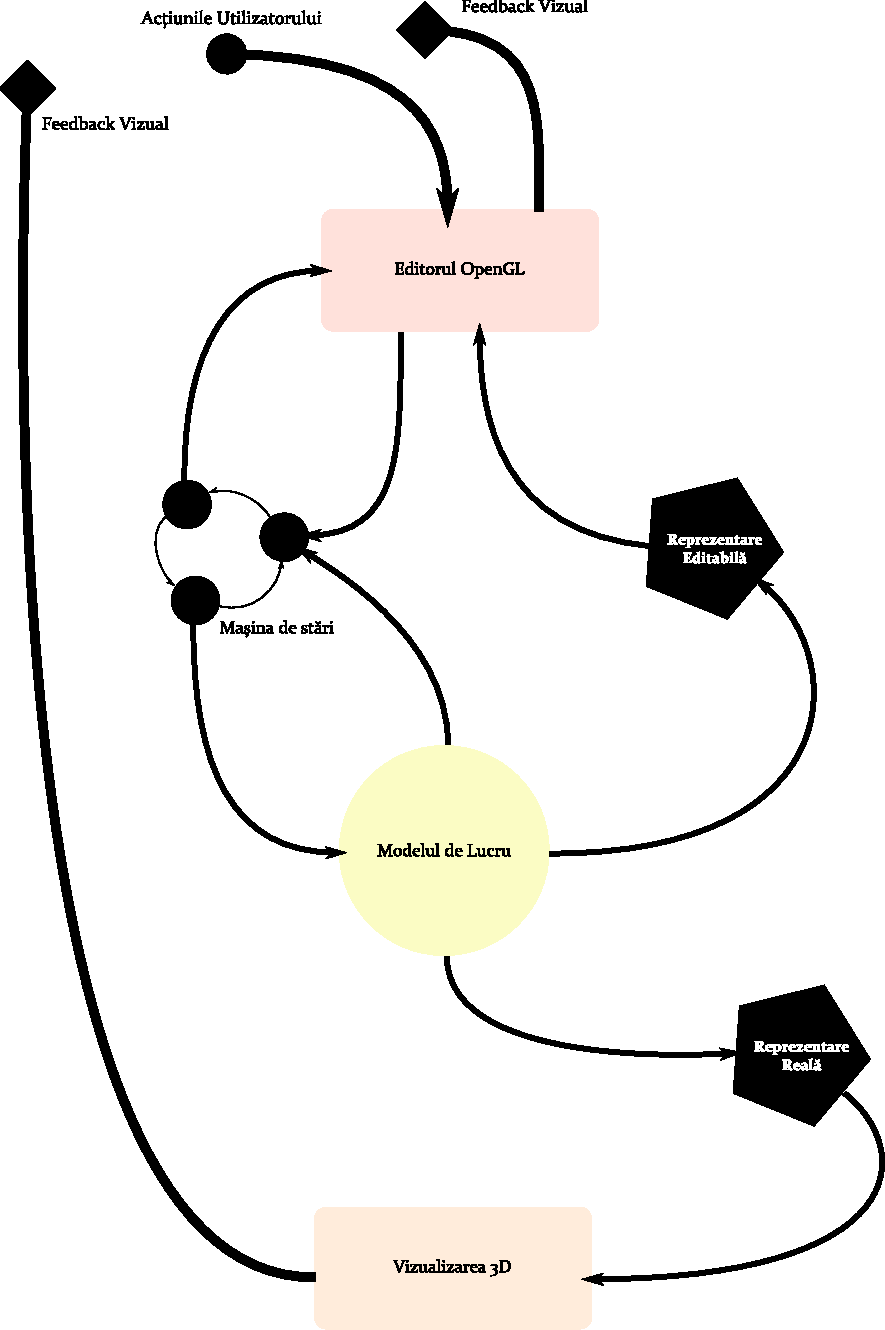
\includegraphics[width=\textwidth]{figures/arh-svg.pdf} \caption{Arhitectura
generală a aplicaţiei}
  \label{figure:arh}
\end{center}
\end{figure}

Proiectată privind către viitor, aplicaţia noastră oferă posibilitatea 
extinderii pe viitor în numeroase direcţii de dezvoltare. Am construit o 
platformă solidă pe baza căreia se poate dezvolta o aplicaţie CAD de un nivel 
comparabil cu a altor aplicaţii de acest tip.

Vom orienta prezentarea noastră în două direcţii. Întîi ne vom concentra asupra 
modelului de lucru. El reprezintă inima proiectului, un concept care uneşte în 
el toate capacităţile acestui proiect. Apoi vom trece la descrierea interfeţei 
cu utilizatorul, a cărei concepţie în sine prezintă o considerăm remarcabilă şi 
reprezintă o bază pentru dezvoltări ulterioare.

În Figura \ref{figure:arh} am făcut o reprezentare schematică a celor ce vor fi
enunţate mai jos, a structurii aplicaţiei şi a principalelor sale componente.

\section{Modelul de lucru}

\begin{definition}
\label{define:model}
Numim \textbf{Model de lucru} reprezentarea într-o colecţie de obiecte Java a 
unei structuri arhitecturale ce poate fi modelată cu ajutorul acestui proiect.
\end{definition}

Modelul de lucru este o reprezentare a unei structuri pe care proiectantul 
doreşte să o reprezinte cu această unealtă într-o formă pe care programul o 
poate recunoaşte şi o poate reface cît mai fidel cu modelul real imaginat de 
proiectant.

\begin{definition}
\label{define:primitive}
Numim \textbf{Primitivă} unitatea structurală şi funcţională a Modelului de 
lucru. O primitivă poate fi o colecţie de alte primitive. De asemenea, o 
primitivă este un element ce poate fi materializat atît la nivel logic cît şi 
într-o reprezentare grafică.
\end{definition}

Primitivele sunt analogiile entităţilor logice în care un model real poate fi 
divizat pentru a-l reprezenta structurat. În seria de primitive ce pot apare în 
modelul logic pot exista primitive care nu au un analog imediat în lumea reală.

\begin{statement}
Modelul logic în totalitatea lui este o Primitivă.
\end{statement}

Plecînd de la aceste două noţiuni, vom încerca să prezentăm întreaga structură 
a Modelului de lucru şi modul în care acesta interacţionează cu aplicaţia în 
sine.

În esenţă, o primitivă este orice poate fi desenat. De aceea, la rîndul său 
modelul este o primitivă. Introducem două direcţii în care modelul poate fi 
reprezentat.

\begin{definition}
\label{define:realRender}
Numim \textbf{Reprezentare Reală} o materializare strictă în comenzi 
Java / OpenGL a unei reprezentări schematice tridimensionale a unei Primitive, 
realizată cu scopul formării unei imaginii asupra rezultatului final al 
construcţiei fizice a entităţii logice din spatele acelei primitive. 
\end{definition} Modelul tridimensional este deci cea mai apropiată formă de 
realitate pe care acest proiect o va reda pentru utilizatorii săi.

\begin{definition}
\label{define:editorRender}
Numim \textbf{Reprezentare Editabilă} o materializare strictă în comenzi 
Java / OpenGL a unei reprezentări schematice bidimensionale a unei Primitive, 
realizată cu scopul identificării vizuale a primitivelor şi accesării facilă 
prin intermediul unui editor a proprietăţilor primitivelor.
\end{definition}

Reprezentarea Editabilă este apropiată ca raţiune figurilor din desenul tehnic, 
şi de aceea identitatea lor vizuală este la rîndul ei asemănătoare acelor 
figuri. Alegerea acestor noţiuni este în strictă corelaţie cu detaliile de 
implementare ale aplicaţiei, care le vom detalia în următorul capitol. Pentru a 
ne face o idee despre cum aceste două reprezentări se potrivesc peste model, 
vom spune că reprezentarea modelului de lucru este juxtapunerea tuturor 
reprezentărilor celorlalte primitive existente în model, în ambele 
reprezentări. Desigur, asta implică că modelul în sine nu este decît un simplu 
container logic pentru toate celelalte componente ale aplicaţiei.

\subsection{Tipuri de primitive}
\label{section:primitives}
Alegerea setului de primitive de care va dispune această aplicaţie a fost o 
sarcină dificilă. Timpul de implementare este în directă corelaţie cu volumul 
de primitive care trebuiesc implementate.

Vom lăsa ca un exerciţiu viitor adăugarea de noi primitive care ar fi de un 
real ajutor utilizatorului acestei aplicaţii. Setul ales este considerat de 
autor ca fiind suficient pentru a oferi un set de funcţionalităţi de bază 
utilizabile pentru această aplicaţie şi destul de variate pentru a scoate în 
evidenţă potenţialul de creştere al acestui proiect.

\subsubsection{Ziduri şi Colţuri de Ziduri}

Elementele constructive esenţiale ale unei structuri sunt zidurile. Ele 
delimitează forma şi suprafaţa construcţiei, avînd un impact crucial asupra 
preţului de construcţie şi facilităţile ce vor putea fi oferite de acea 
construcţie.

Colţurile sunt un tip de primitivă indirect disponibilă proiectantului. Unirea 
capetelor a două ziduri se poate face printr-un colţ, care introduce de fapt o 
legătură permanentă între marginile acelor două ziduri. Constrîngerea este una 
punctuală, zidurile putînd avea orice orientare în cadrul modelului atîta timp 
cît sunt conectate la un colţ. Colţurile pot fi privite ca nişte puncte într-un 
plan.

Orice zid este conectat la două colţuri, \textbf{Colţul de Start} şi 
\textbf{Colţul de Stop}. Astfel poziţionat, lungimea şi orientarea unui zid 
este dictată de poziţia celor două colţuri. Astfel, un zid poate fi privit ca 
un segment ce leagă oricare două puncte (colţuri) dintr-un plan.

\subsubsection{Caracteristici de Ziduri}
\label{section:features}

\begin{definition}
\label{define:feature}
Numim \textbf{Caracteristică a unui Zid} orice Primitivă ce este asociată în 
mod direct cu un zid.
\end{definition}

Toate Caractersticile sunt constrînse poziţional în lungimea zidului. Ele 
adaugă elemente suplimentare modelului care sunt strict legate în realitate de 
existenţa unui zid. Exemple tipice de caracterstici ce elucidează şi mai bine 
ce reprezintă o caracteristică ar fi:

\begin{itemize}
  \item Fereastră
  \item Uşă
\end{itemize}
  
\subsubsection{Decoraţiuni}
  
\begin{definition}
\label{define:decoration}
\textbf{Decoraţiunile} sunt Primitive care nu au legătură strictă cu structura 
construită, însă oferă un plus de realism şi poate sugera viitoarea destinaţie 
a diferitelor spaţii din model.
\end{definition}
  
\begin{itemize}
  \item Canapea
  \item Masă
\end{itemize}

Dintre aceste Decoraţiuni, unele dintre ele vor fi implementate ca şi 
Caracterstici, datorită constrîngerii lor reale de a apărea pe un zid.
\subsection{Aspecte ale modelului}

\begin{definition}
\label{define:model-aspect}
Numim \textbf{Aspect al Modelului de Lucru} orice formă de interpretare a unei 
primitive aflate într-un model de lucru care nu are legătură cu modelul şi 
structura sa, dar ajută alte componente ale aplicaţiei în a interacţiona cu 
acesta.
\end{definition}

Pentru modelarea funcţionalităţii editorului, orice Primitivă 
(\ref{define:primitive}) este considerată ca un element ce poate fi desenat 
într-un editor. Fiecare Primitivă trebuie să specifice modul în care ea urmează 
să fie desenată în spaţiul bidimensional al editorului.

Unele primitive sunt desenate direct de către model, altele, cum ar fi 
Caracteristicile (\ref{define:feature}), ale căror desenare intră în 
sarcina zidului din care fac parte.

Acest aspect al modelului reprezintă materializarea \textbf{Reprezentării 
Editabile} (\ref{define:editorRender}).

Un alt aspect adăugat modelului este \textbf{Selectabilitate}.

\begin{definition}
\label{define:selectable}
Orice Primitivă care din punct de vedere al interfeţei editorului poate fi 
selectat prin diverse metode de utilizator se spune că este 
\textbf{selectabilă}, sau că are un aspect de \textbf{Selectabilitate}.
\end{definition}

Primitivele pot reacţiona la schimbarea stării lor de selectabilitate şi la 
rîndul său editorul poate trata evenimentul schimbării selecţiei în funcţie de 
implementarea dorită.

În fine, ultimul aspect al modelului necesar implementării editorului este cel 
de \textbf{Navigabilitate}.

\begin{definition}
\label{define:hoverable}
În momentul în care mausul trece deasupra unei 
astfel de componente, ea poate reacţiona prin evenimente implementate la 
nivelul editorului, avînd astfel aspectul de \textbf{Navigabilitate}.
\end{definition}

Multe Primitive folosesc această proprietate pentru a-şi schimba starea de 
selectare. Fiecare Primitivă selectabilă defineşte o stare proprie în care
editorul va trece în momentul în care primitiva respectivă este selectată. Dacă
primitiva nu defineşte o astfel de stare, atunci editorul rămîne în starea de
navigare.

\section{Editorul OpenGL}
\label{section:opengl-editor}

Înainte de a fi un editor pentru Modelul de Lucru (\ref{define:model}), 
editorul OpenGL dezvoltat de noi este un punct de plecare foarte bun pentru 
orice editor care necesită folosirea facilităţilor OpenGL. Vom încerca să 
descriem succint arhitectura editorului, evidenţiind caracteristicile generice 
cît şi particularizările de suprafaţă care au fost necesare pentru integrarea 
cu funcţionarea dorită.

Editorul este în principiu o suprafaţă de desenare OpenGL cu aspect 
bidimensional ce poate interacţiona cu utilizatorul prin intermediul interfeţei 
oferite de RCP, adică evenimentele ale mausului, ale tastaturii, ale 
vizualizărilor de structură şi de proprietăţi, despre care vom aminti mai jos.


\subsection{Editorul ca maşină de stări}
\label{section:machine}

Editorul OpenGL funcţionează ca o maşină de stări. Editorul suportă 
înregistrarea stărilor noi şi controlează viaţa tuturor stărilor înregistrate 
în stiva sa de stări.

La un moment dat o singură stare este activă. O stare activă poate controla 
toate evenimentele pe care le primeşte editorul şi poate să introducă noi stări 
în stivă sau să modifice modelul în funcţie de evenimentele care au avut loc. 
Starea decide cînd viaţa ei a luat sfîrşit. Această decizie este comunicată 
editorului care apoi deînregistrează starea din stivă.

În Tabela \ref{table:editor-states} vom prezenta ciclul de viaţă al unei stări. 
Acest model de ciclu de viaţă a fost stabilit în funcţie de necesităţile 
editorului OpenGL, pentru a-i permite acestuia să interacţioneze sincron cu 
schimbările de stare ce pot fi controlate asincron de către evenimentele 
aplicaţiei.

Dintr-o anumită privinţă, acest ciclu de stare poate fi privit ca o serie de 
meta-stări ale aplicaţiei (i.e. stări ale stărilor).

\begin{table}[htp] \caption{Ciclul de viaţă al stărilor Editorului OpenGL
\label{table:editor-states}}
\begin{tabular}{|\col{0.23}|\col{0.73}|}

\hline FRESH & La construcţia unei stări ciclul de viaţă este setat în poziţia 
FRESH. Editorul va citi orice stare setată pe acest mod şi o va seta ca şi 
stare activă, înregistrînd toate rutinele de tratare a evenimentelor pentru 
această stare în cadrul editorului. Starea curentă este setată ca activă şi 
modul ei este trecut în RUNNING. Starea activă anterioară este trecută pe modul 
SLEEPING. \\

\hline RUNNING & După ce editorul iniţializează o stare, ea este în modul 
RUNNING. În acest mod starea primeşte toate evenimentele editorului. Decizia de 
a părăsi această stare se poate lua după două criterii. a) La discreţia stării 
în sine, prin trecerea în modul TERMINATED sau b) la discreţia editorului, în 
momentul sosirii unei noi stări FRESH, cînd starea curentă trece în SLEEPING. \\

\hline SLEEPING & Toate stările care au fost oprite de editor la apariţia unei 
stări noi se adună într-o stivă şi modul lor este trecut în SLEEPING. Ele pot 
sta în acest mod un timp nedefinit şi pot să nu-l părăsească niciodată. Ele pot 
reveni la starea RUNNING în momentul în care se află la vîrful stivei şi starea 
activă trece în modul TERMINATED. Atunci editorul automat va muta starea din 
capul stivei ca stare activă şi ea va deveni RUNNING. De aceea rutina de 
tratare a tranziţiei în RUNNING cît şi rutina de tratare în starea TERMINATED 
trebuie să aibă în vedere posibilitatea rulării de mai multe ori pentru aceeaşi 
stare (i.e. să nu trateze iniţializări, care se fac în mod normal în starea 
FRESH) \\

\hline TERMINATED & Odată ce starea consideră că şi-a încheiat activitatea, ea 
poate alege să treacă în modul TERMINATED. Odată ajunsă în acest mod, starea va 
fi deînregistrată din lista de captare a evenimentelor editorului şi va fi 
scoasă permanent din lista stărilor editorului.\\

\hline
\end{tabular}
\end{table}

Stările editorului sunt folosite pentru a manipula modelul de lucru. Ele pot 
adăuga şterge sau schimba diverse proprietăţi ale primitivelor aflate în model. 
Din acest motiv, stările sunt strict asociate cu diversele tipuri de primitive 
din model.

Există o stare nativă a editorului, anume starea de navigare. Este singura stare
definită aici care nu se termină niciodată, şi este pornită automat de către
editor la iniţializarea sa. Starea de navigare este responsabilă de
administrarea diverselor proprietăţi ale obiectelor, ea fiind cea care ia
decizia -- şi în acelaşi timp informează -- fiecare proprietate de starea sa de
acoperire cu mausul. De asemenea, ea porneşte mecanismul de selecate a
obiectelor şi de trecere în starea predefinită de fiecare obiect care poate fi
selectat dintr-o scenă.

Starea de selectare este o stare specială în care editorul trece atunci cînd un
obiect este selectat cu ajutorul diverselor metode puse la dispoziţie de Eclipse
RCP. Starea de selectare este folosită de Colţuri, spre exemplu, pentru a iniţia
procedura de transformare prin deplasare a mausului, mişcare prin care poziţia
Colţului este modificată. Starea de selecţie a colţului trebuie să aibă în
vedere -- precum toate celelalte stări de selecţie -- că selecţia poate avea mai
multe surse şi comportamentul său predefinit -- de a transporta cu ajutorul
mausului colţul -- nu este valid decît în cazul selecţiei cu ajutorul mausului.
Această discriminare se face cu ajutorul stării de acoperire cu mausul a
Colţului respectiv\footnote{Dacă mausul nu este deasupra componentei, înseamnă
că selecţia avut loc prin alte mecanisme, şi atunci se anulează procedura de
mutare a colţului}.

\subsection{Capacităţi asincrone}

Editorul OpenGL este optimizat pentru motorul asincron de sincronizare, 
desenare şi tratare a evenimentelor ale aplicaţiilor Eclipse RCP. Deşi vom 
intra în detalii în capitolul \ref{chapter:impl}, amintim doar aici că într-o 
singură aplicaţie se pot edita oricîte Modele de Lucru, fără nici un impact 
asupra unuia dintre ele şi fără interferenţe de nici un fel atît în logica 
modelului cît şi în ciclul de randare.

\section{Vizualizarea 3D OpenGL}
\label{section:view}

După cum am văzut în secţiunea \ref{section:opengl-editor}, Editorul OpenGL 
serveşte la manipularea Modelului de Lucru (\ref{define:model}) şi a 
proprietăţilor diverselor Primitive (\ref{define:primitive}) din acest Model. 
Sarcina vizualizării tridimensionale a modelului cade în măinile componentei 
despre care vom discuta în această secţiune.

Diferenţa principală dintre Editor şi Vizualizare este că cea din urmă nu 
permite interacţiunea cu proprietăţile modelului, ci doar proiecţia lor într-o 
lume tridimensională. Proiecţia se face într-o scenă văzută în perspectivă şi 
cu toate obiectele desenate prin contur cu muchiile din spate ascunse. Modelul 
poate fi explorat cu ajutorul mausului, însă nu se poate interacţiona în nici 
un fel similar cu capacităţile editorului.

\subsection{Aspectul de desenare reală}

La rîndul său, Vizualizarea 3D introduce un aspect (\ref{define:model-aspect}) 
asupra Modelului de Lucru. Acest aspect este cel de \textbf{desenare reală}. 
Deşi structura ierhahică a liniei de randare este similară cu cea a aspectului 
de randare pentru editare, există o singură diferenţă semnificativă.

Pentru randarea scenei cu contur ascunzînd muchiile din spate, OpenGL necesită 
ca scena să fie randată în două treceri. Prima trecere reprezintă volumele de 
randare şi în a doua trecere se desenează contururile.

În principiu, aspectul de desenare reală trebuie să aibă în vedere optimizarea 
celor două treceri pentru a obţine doar acele contururi care sunt de interes 
pentru utilizator, fără a marca toate poligoanele din scenă.

\subsection{Conexiunea cu Editorul OpenGL}

Precum Editorul OpenGL, Vizualizarea 3D OpenGL are şi ea ample capacităţi 
asincrone, răspunzînd la solicitările editorului şi putînd servi simultan 
nevoile a mai multor editoare. Platforma RCP forţează ca orice vizualizare să 
existe o singură dată în interfaţa grafică. Prin această limitare se impune ca 
Vizualizarea 3D să reprezinte doar modelul aflat în Editorul activ la un moment 
dat.

De asemenea, Vizualizarea 3D are capacitatea de a reprezenta orice modificare
are loc în Modelul de Lucru în timp real, în momentul în care datele parţiale
sunt salvate în Model.

\section{Vizualizarea structurii modelului}

Eclipse RCP oferă o vizualizare predefinită pentru descrierea structurii 
conţinutului unui editor\footnote{cunoscută în documentaţia Eclipse ca 
\textit{Content Outline View}}. În cazul de faţă, conţinutul logic al 
editorului îl reprezintă tocmai modelul, şi astfel o reprezentare a structurii 
modelului a fost furnizată pentru această vizualizare.

În cadrul acestei vizualizări utilizatorul poate modifica selecţia curentă în
editor şi poate afla informaţii despre poziţia diverselor componente ale
modelului. Afişarea acestor informaţii este în strictă legătură cu sursa de
selecţie.


\subsection{Sursa de selecţie. Descriptorul de conţinut}

Orice Pagină Eclipse\footnote{Paginile sunt descrise în Secţiunea
\ref{section:workbench}} poate avea o sursă de selecţie. O sursă de selecţie
este un concept abstract care vine asupra conţinutului unui editor pentru a
ajuta sincronizarea afişării informaţiilor în diverse vizualizări care sunt
implementate în program.

Special pentru scopurile Vizualizării 3D şi a Vizualizării de structură despre
care amintim acum, am definit o sursă de selecţie strict legată de modelul de
lucru din editor.

Această sursă de selecţie implementează conceptul abstract definit în Eclipse şi
îl adaptează nevoilor modelului nostru. El este capabil şi conştient de
diversele tipuri de Primitive care există în model şi poate distinge între
stările acestora.

Acesta reprezintă deci un descriptor de conţinut al editorului care este folosit
de către Pagina Eclipse pentru sincronizarea diverselor componente ale
interfeţei grafice.

\section{Particularizarea Platformei Eclipse}

\subsection{Facilităţile de creare de noi fişiere şi proiecte}

Aplicaţia noastră vine cu facilităţi pentru uşurarea creării de noi modele de
editare şi pentru crearea de proiecte noi ce vor organiza modelele create de
utilizator. Pentru particularizarea acestora, am folosit modele predefinite care
vin cu aplicaţia Eclipse.

Funcţiile acestor automatizări ale creării de proiecte şi fişiere sunt crearea 
de noi astfel de componente cu setările potrivite pentru utilizarea cu această 
aplicaţie. În particular, proiectul nu are nici o caracteristică deosebită însă 
fişierele trebuie să aibă întotdeauna extensia ocm\footnote{abrev. 
\textit{OpenCad.org Model}}.

\subsection{Perspectiva de lucru}

După cum am prezentat anterior\footnote{În secţiunea \ref{section:workbench}},
Perspectivele oferă o aşezare pentru toate componentele din Pagina unui
Workbench.

Varianta particularizată pentru acest proiect porneşte cu vizualizarea de
navigare în partea de stînga sus, cu Vizualizarea 3D în stînga jos şi cu
editorul modelului în partea dreaptă.

\subsection{Butoanele de acţiuni}

Pentru diverse acţiuni din cadrul aplicaţiei am adăugat butoane care iniţiază
executarea comenzilor respective. În general, butoanele servesc operaţiunilor
de modificare a structurii modelului. Există astfel butoane pentru adăugarea de
ziduri, ferestre, uşi, etc.

		\chapter{Implementare}
\label{chapter:impl}

În acest capitol vom prezenta detaliile implementării acestui proiect. Se va 
trece prin structura de clase, fluxul datelor în aplicaţie, mutaţiile Modelului 
de Lucru (\ref{define:model})  şi funcţionarea componentelor de interfaţă,
editorul OpenGL şi Vizualizarea 3D, prezentate în secţiunile
\ref{section:opengl-editor}, respectiv \ref{section:view}.

\section{Structura claselor}

Fiecare dintre componentele arhitecturale descrise la capitolul 
\ref{chapter:arh} sunt materializate în implementarea efectivă printr-un set de 
clase bine definite şi bine separate ca logică şi structură de celelalte 
componente ale aplicaţiei.

\subsection{Modelul de Lucru}

\subsubsection{Primitive}
Clasa de bază a modelului de lucru este clasa Primitive. Desigur, este o
materializare a conceptului de Primitivă (\ref{define:primitive}). Aceasta este o clasă 
abstractă care nu introduce nici un comportament singular, însă marchează 
nevoie de implementare pentru intefeţele EditorRenderable şi RealRenderable, 
necesare celor două vizualizări, cum vom vedea la secţiunile 
\ref{section:impl-editor} şi \ref{section:impl-view}.

Din clasa Primitive sunt extinse clasele concrete Corner, Wall şi
toate clasele ce implementează Decoraţiunile (\ref{define:decoration}). Fiecare
din aceste clase implementează metodele definite în interfeţele amintite mai
sus.

Tot din clasa Primitive se desprinde şi clasa WallFeature, o materializare a
conceptului de Caracterstică de Ziduri (\ref{define:feature}). Din ea la rîndul
ei se concretizează clasele Door, Window, Inset, Outset, Tunnel, implementări
ale diverselor caracteristici amintite în \ref{section:primitives}.

\subsubsection{Corner}

Clasa Corner reprezintă una din puţinele Primitive care nu sunt direct
disponibile utilizatorului aplicaţiei. Ea serveşte strict poziţionării Zidurilor
şi prin aceasta editorul nu le oferă o importanţă deosebită printr-o
individualizare în cadrul interfeţei, reducînd astfel solicitarea asupra curbei
de învăţare a utilizatorului.

Clasa Corner, pe lîngă implementarea comportamentului de desenare pentru
proiectate (\ref{define:editorRender}) şi de desenare reală
(\ref{define:realRender}), aderă şi la comportamentele de Selectabilitate
(\ref{define:selectable}) şi de Navigabilitate (\ref{define:hoverable}).

		\chapter{Concluzii}

Vom încerca să prezentăm succint, în această ultimă parte, o serie de concluzii
şi observaţii la care am ajuns în procesul de dezvoltare a acestui proiect şi în
momentul finalizării sale.

În primul rînd, trebuie să subliniem rolul covîrşitor pe care l-a avut Eclipse
Rich Client Platform (\ref{section:rcp}) în acest proiect. Aşa cum ne aşteptam,
platforma în cauză reprezintă o bază solidă pentru dezvoltarea aplicaţiilor
desktop şi, în ciuda specializării sale pentru unelte de dezvoltare IDE pentru
programare, s-a dovedit a fi destul de generică pentru a oferi suport pentru
tipul de aplicaţie care l-am avut în vedere.

Integrarea Eclipse RCP şi a OpenGL a funcţionat la nivelul aşteptărilor, oferind
o bază reală de dezvoltare, identică -- dacă nu mai puternică -- cu alte soluţii
pentru grafica tridimensională. Plugin-ul pentru OpenGL dezvoltat de Fundaţia
Eclipse reprezintă deci un început bun pentru aducerea capacităţilor 3D în
aplicaţii dezvoltate cu şi pentru Eclipse.

Considerăm că aplicaţia de faţă a reuşit să întîlnească prospectele iniţiale în
ceea ce priveşte uşurinţa de folosire şi integrarea cu alte unelte Eclipse.
Funcţionalităţile implementate pot fi duse mai departe prin puterea de extensie
a platformei şi prin nivelul de abstracţie la care acest proiect a fost
proiectat. 

În ceea ce priveşte utilitatea aplicaţiei, credem că poate reprezenta un punct
de pornire pentru o unealtă de proiectare de nivelul altor astfel de aplicaţii
consacrate, şi poate fi folosită şi în forma sa actuală de către proiectanţii de
ansambluri arhitectonice.

Pentru viitor, există posibilitatea dezvoltării în continuare a acestei soluţii,
oferind astfel din ce în ce mai multe facilităţi şi o interfaţă mai puternică
pentru viitorii utilizatori.

\clearpage
	\pagenumbering{roman}
	\bibliographystyle{plain}
	\bibliography{thesis}
\end{document}